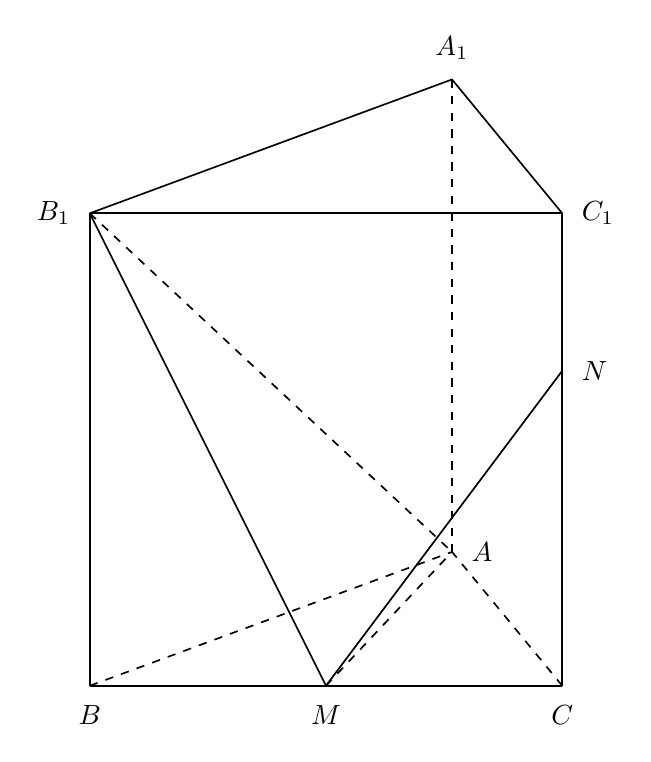
\begin{tikzpicture}[x=1cm,y=1cm,line width=0.6pt]
\coordinate (B) at (0,0);
\coordinate (M) at (3,0);
\coordinate (C) at (6,0);
\coordinate (B1) at (0,6);
\coordinate (C1) at (6,6);
\coordinate (A) at (4.6,1.7);
\coordinate (A1) at (4.6,7.7);
\coordinate (N) at (6,4);
% solid frame and auxiliaries
\draw[draw=black] (B) -- (M) -- (C);
\draw[draw=black] (B) -- (B1);
\draw[draw=black] (C) -- (C1);
\draw[draw=black] (B1) -- (C1);
\draw[draw=black] (B1) -- (A1) -- (C1);
\draw[draw=black] (B1) -- (M);
\draw[draw=black] (M) -- (N);
% hidden / interior dashed
\draw[draw=black,dashed] (B) -- (A);
\draw[draw=black,dashed] (M) -- (A);
\draw[draw=black,dashed] (C) -- (A);
\draw[draw=black,dashed] (B1) -- (A);
\draw[draw=black,dashed] (A1) -- (A);
% labels
\node[anchor=north,font=\normalsize] at ([yshift=-0.12cm]B) {$B$};
\node[anchor=north,font=\normalsize] at ([yshift=-0.12cm]M) {$M$};
\node[anchor=north,font=\normalsize] at ([yshift=-0.12cm]C) {$C$};
\node[anchor=east,font=\normalsize] at ([xshift=-0.12cm]B1) {$B_{1}$};
\node[anchor=west,font=\normalsize] at ([xshift=0.12cm]C1) {$C_{1}$};
\node[anchor=south,font=\normalsize] at ([yshift=0.12cm]A1) {$A_{1}$};
\node[anchor=west,font=\normalsize] at ([xshift=0.12cm]A) {$A$};
\node[anchor=west,font=\normalsize] at ([xshift=0.12cm]N) {$N$};
\end{tikzpicture}